\subsection{Requirements Verification}\label{sec:srsVV}
The goal of requirements verification is to evaluate the Software Requirements
Specification (SRS) for correctness, consistency, completeness, readability,
testability, and traceability. This corresponds to the requirements evaluation
and traceability analysis tasks in Section 9.2 of IEEE Std
1012-2016~\citep{vvIEEE}.

\paragraph{Method} The SRS verification plan relies on peer review/document
inspection with the following stages:
\begin{enumerate}

    \item Preparation: Participants review the SRS document with respect to
    their assigned role and goals (Table~\ref{tab:rolesSRS})

    \item Meeting: Participants meet to discuss findings, potential issues, and
    proposed action plans to address them

    \item Rework: The SRS author(s) revise the document to address raised
    issues, guided by the proposed action plans

    \item Follow Up: Participants verify that raised issues have been addressed
    satisfactorily

\end{enumerate}

A recording device might be used to capture meeting proceedings in place of
physical note taking so that all participants can focus on the discussion.

Peer review/inspection begins when there is a new major version of the SRS
document.

Peer review/inspection ends when reviewers agree that there are no issues that
will likely result in an extensive loss of confidence in \progname{} (e.g.
barrier to adoption by primary stakeholders).

\paragraph{Roles and Responsibilities} To assist in the achievement of their
assigned goals (Table~\ref{tab:rolesSRS}) using peer review/document inspection:
\begin{itemize}

    \item Primary team members are responsible for ensuring that reviewers have
    the necessary materials, moderating the inspection process and reading
    through the SRS document during the meeting(s)

    \item Secondary and tertiary members are reviewers whom are responsible for
    reviewing the SRS document prior to the meeting(s) so that they are prepared
    to discuss it with the team

\end{itemize}

\paragraph{Inputs}
\begin{itemize}

    \item Software Requirements Specification for \progname{}: A Computational
    Model of Emotion for Enhancing Non-Player Character Believability in Games

    \item Concept Summary for \progname{}: A Computational Model of Emotion for
    Enhancing Non-Player Character Believability in Games

    \item References used to generate primary stakeholder requirements

    \item Review guide for \progname{}'s SRS
    (Appendix~\ref{appendix:srsInspection})

\end{itemize}

\paragraph{Outputs}
\begin{itemize}

    \item Objective evidence to assess the verification of the SRS

    \item Objective evidence that the requirements are complete, correct,
    accurate, and testable

    \item Objective evidence that the requirements are traceable to
    \progname{}'s concept summary and intended use and user needs

    \item Objective evidence that the SRS is readable

    \item Input to Master Test Report (MTR)

\end{itemize}

\paragraph{Estimated Completion Time} Four (4) weeks

Due to the document's size, SRS peer review/inspection is divided into parts.
Only one part is tested per week to reduce participant fatigue:
\begin{itemize}

    \item Part 1: Introduction (Section~2), General System Description
    (Section~3)

    \item Part 2: Problem Description (Section~4.1), Solution Characteristics
    Specification: Emotion Theories and Models (Section~4.2.1), Assumptions
    (Section~4.2.2), Conceptual Models (Section~4.2.3), Theoretical Models
    (Section~4.2.4)

    \item Part 3: Solution Characteristics Specification: General Definitions
    (Section~4.2.5), Data Definitions (Section~4.2.6), Type Definitions
    (Section~4.2.7), Instance Models (Section~4.2.8), Data Constraints
    (Section~4.2.9), Properties of a Correct Solution (Section~4.2.10)

    \item Part 4: Requirements (Section~5), Future Changes (Section~6),
    Traceability Matrices and Graphs (Section~7)

\end{itemize}

\begin{figure}[!h]
    \centering
    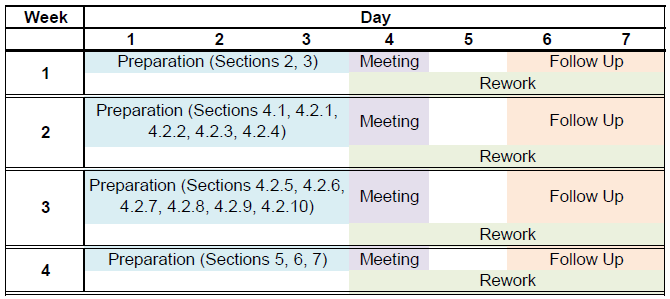
\includegraphics[width=0.9\linewidth]{figures/Requirements_Schedule.png}
\end{figure}